% This file was created with tikzplotlib v0.10.1.
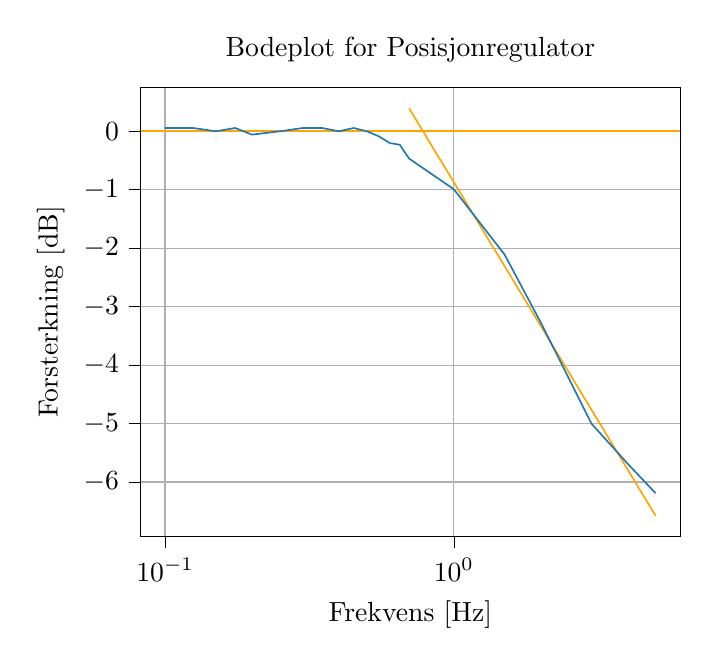
\begin{tikzpicture}

\definecolor{darkgray176}{RGB}{176,176,176}
\definecolor{orange}{RGB}{255,165,0}
\definecolor{steelblue31119180}{RGB}{31,119,180}

\begin{axis}[
log basis x={10},
tick align=outside,
tick pos=left,
title={Bodeplot for Posisjonregulator},
x grid style={darkgray176},
xlabel={Frekvens [Hz]},
xmajorgrids,
xmin=0.0822340159426889, xmax=6.08020895329329,
xminorgrids,
xmode=log,
xtick style={color=black},
xtick={0.001,0.01,0.1,1,10,100},
xticklabels={
  \(\displaystyle {10^{-3}}\),
  \(\displaystyle {10^{-2}}\),
  \(\displaystyle {10^{-1}}\),
  \(\displaystyle {10^{0}}\),
  \(\displaystyle {10^{1}}\),
  \(\displaystyle {10^{2}}\)
},
y grid style={darkgray176},
ylabel={Forsterkning [dB]},
ymajorgrids,
ymin=-6.92696915493292, ymax=0.742898747755512,
yminorgrids,
ytick style={color=black},
ytick={-7,-6,-5,-4,-3,-2,-1,0,1},
yticklabels={
  \(\displaystyle {\ensuremath{-}7}\),
  \(\displaystyle {\ensuremath{-}6}\),
  \(\displaystyle {\ensuremath{-}5}\),
  \(\displaystyle {\ensuremath{-}4}\),
  \(\displaystyle {\ensuremath{-}3}\),
  \(\displaystyle {\ensuremath{-}2}\),
  \(\displaystyle {\ensuremath{-}1}\),
  \(\displaystyle {0}\),
  \(\displaystyle {1}\)
}
]
\addplot [semithick, orange]
table {%
0.0822340159426889 0
6.08020895329329 0
};
\addplot [semithick, orange]
table {%
0.7 0.394268388542402
1.17777777777778 -1.45093493262608
1.65555555555556 -2.65850703298998
2.13333333333333 -3.55769144857336
2.61111111111111 -4.27438234056457
3.08888888888889 -4.87030247038411
3.56666666666667 -5.38034462173227
4.04444444444444 -5.8261713110089
4.52222222222222 -6.22215903826441
5 -6.57833879571981
};
\addplot [semithick, steelblue31119180]
table {%
0.1 0.0565858003772851
0.125 0.0565858003772851
0.15 0
0.175 0.0565858003772851
0.2 -0.0569568574565249
0.25 0
0.3 0.0565858003772851
0.35 0.0565858003772851
0.4 0
0.45 0.0565858003772851
0.5 0
0.55 -0.0855759595855004
0.6 -0.201004763143006
0.65 -0.230103248106495
0.7 -0.466468571652479
1 -0.99117558881648
1.5 -2.11020369539948
2 -3.27004263495321
3 -5.00385959148062
4 -5.68648604322257
5 -6.19260334851798
};
\end{axis}

\end{tikzpicture}
